\documentclass[12pt]{article}

% ===== PACKAGES =====
\usepackage[margin=1.2in]{geometry}
\usepackage{amsmath, amssymb}
\usepackage{graphicx}
\usepackage{xcolor}
\usepackage{pagecolor}
\usepackage{tcolorbox}
\tcbuselibrary{skins, breakable}
\usepackage{sectsty}
\usepackage{float}

% ===== COLORS =====
\definecolor{BG}{HTML}{121212}
\definecolor{FG}{HTML}{F2F2F2}
\definecolor{BLUE}{HTML}{58C4DD}
\definecolor{GREEN}{HTML}{83C167}
\definecolor{GOLD}{HTML}{F0AC5F}
\definecolor{RED}{HTML}{FC6255}

\pagecolor{BG}
\color{FG}

\sectionfont{\color{BLUE}}

\newtcolorbox{boxstyle}{
  colback=black!80,
  colframe=BLUE,
  sharp corners,
  boxrule=0pt,
  left=10pt,right=10pt,top=8pt,bottom=8pt
}

\title{\color{BLUE} ENEE 323 Project 4\\Hilbert Transform \& SSB}
\author{\color{FG} Yahya Mouamil \\ UID: 119873526}
\date{}

\begin{document}
\maketitle

% =========================
\section*{Part (i)}
\begin{boxstyle}
FIR coefficients are antisymmetric about $M=40$. Center value is zero. 
Odd-index structure and $\frac{2}{\pi n}$ decay matches ideal Hilbert transformer.
\end{boxstyle}

\begin{figure}[H]
\centering
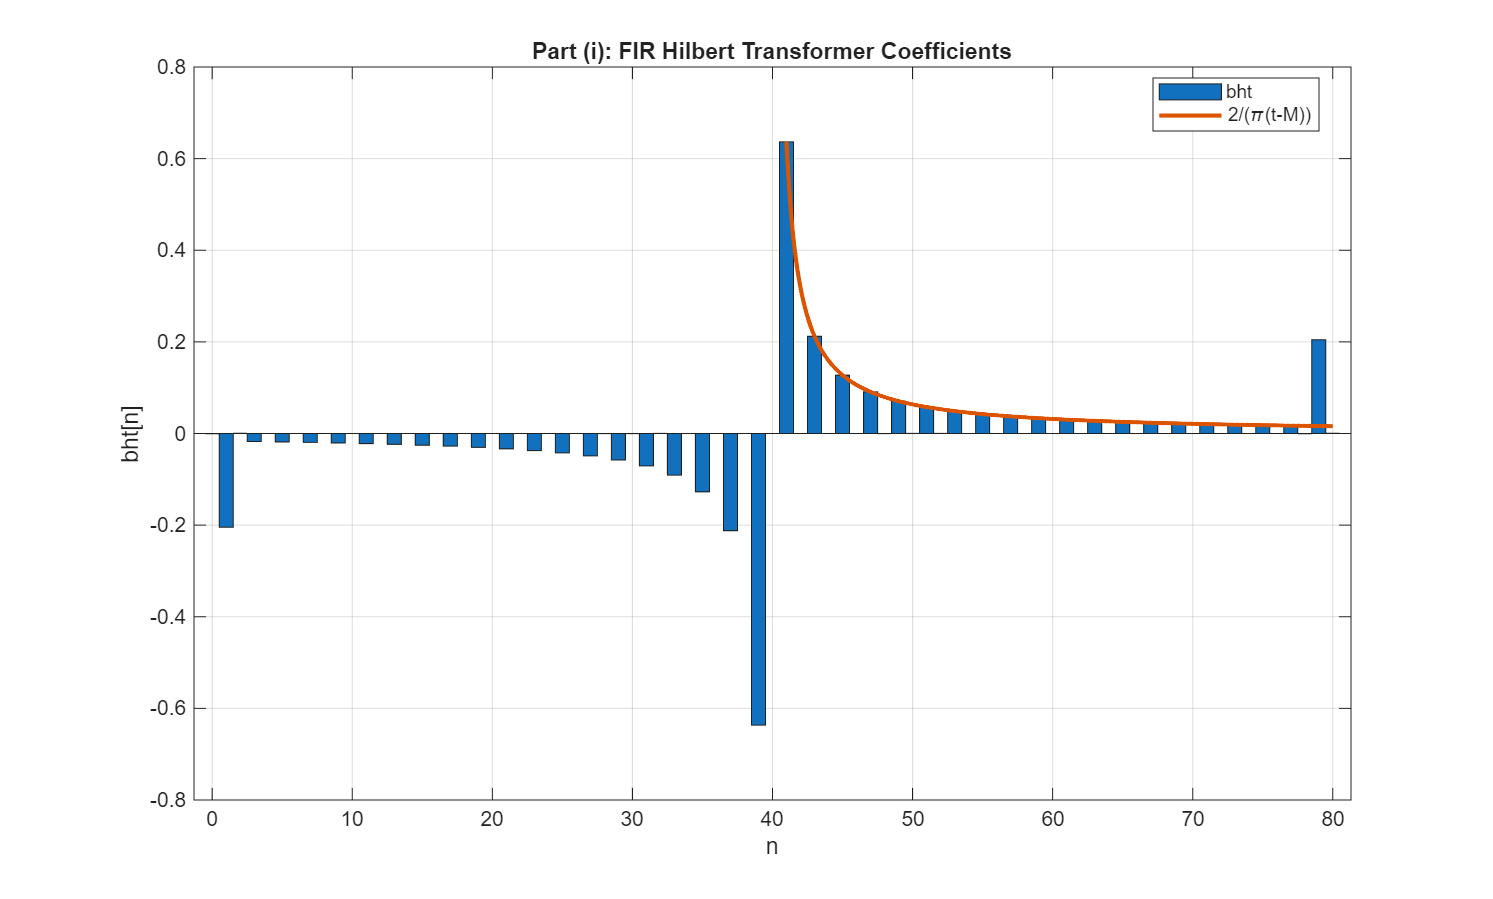
\includegraphics[width=0.85\textwidth]{part1_coefficients.png}
\end{figure}

% =========================
\section*{Part (ii)}
\begin{boxstyle}
Passband: $[800, 15200]$ Hz \\
Ripple: $7.22$ dB \\
Phase slope reflects delay $\approx 40$ samples. \\
Intercept shows $\pm \frac{\pi}{2}$ shift.
\end{boxstyle}

\begin{figure}[H]
\centering
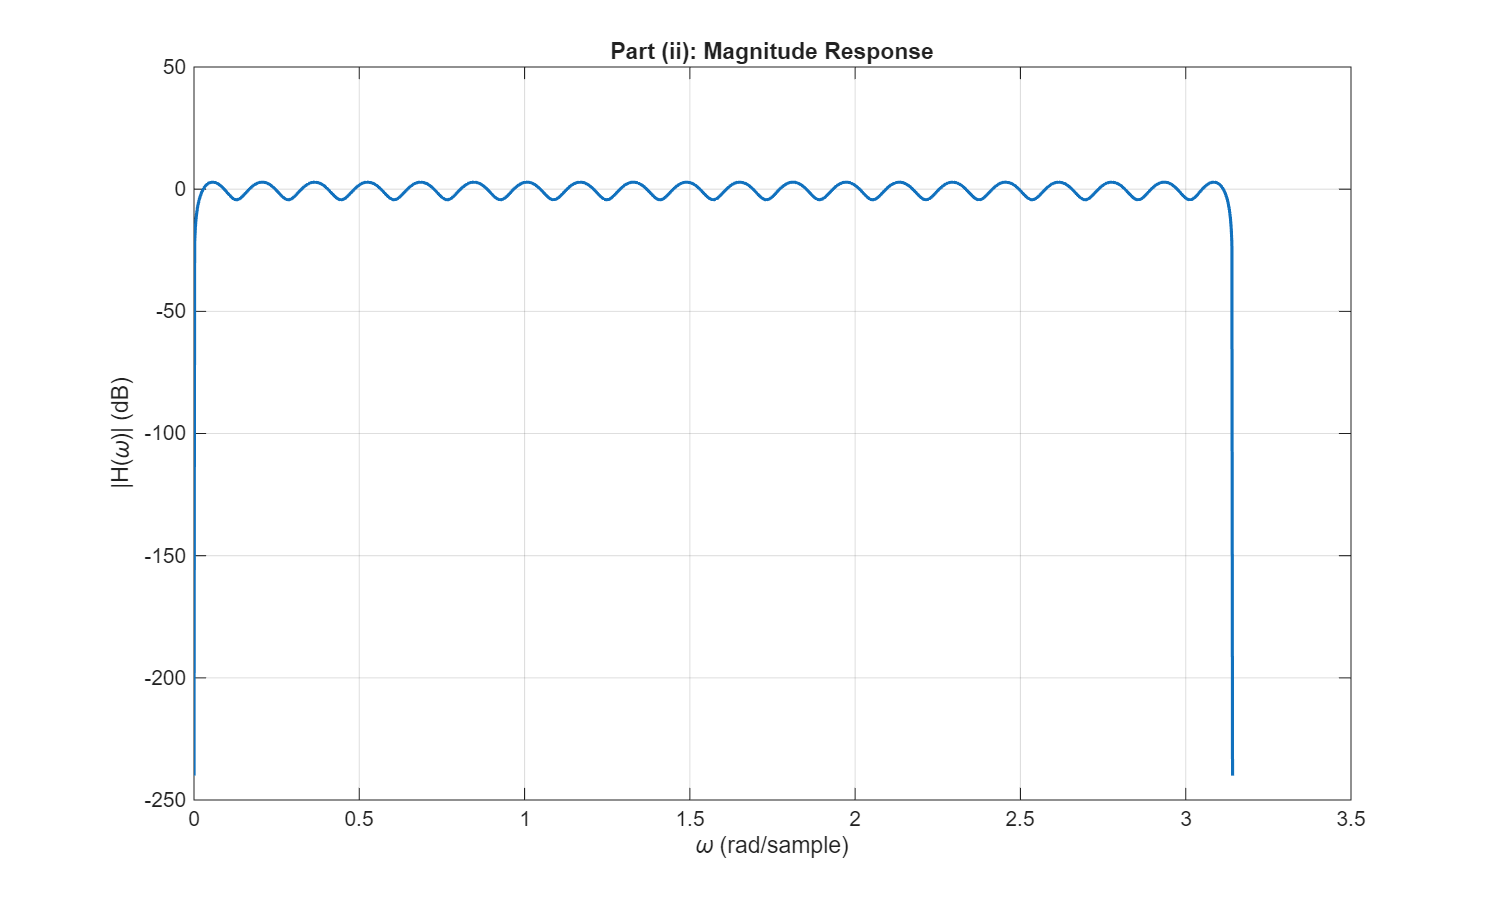
\includegraphics[width=0.85\textwidth]{part2_magnitude.png}
\end{figure}

\begin{figure}[H]
\centering
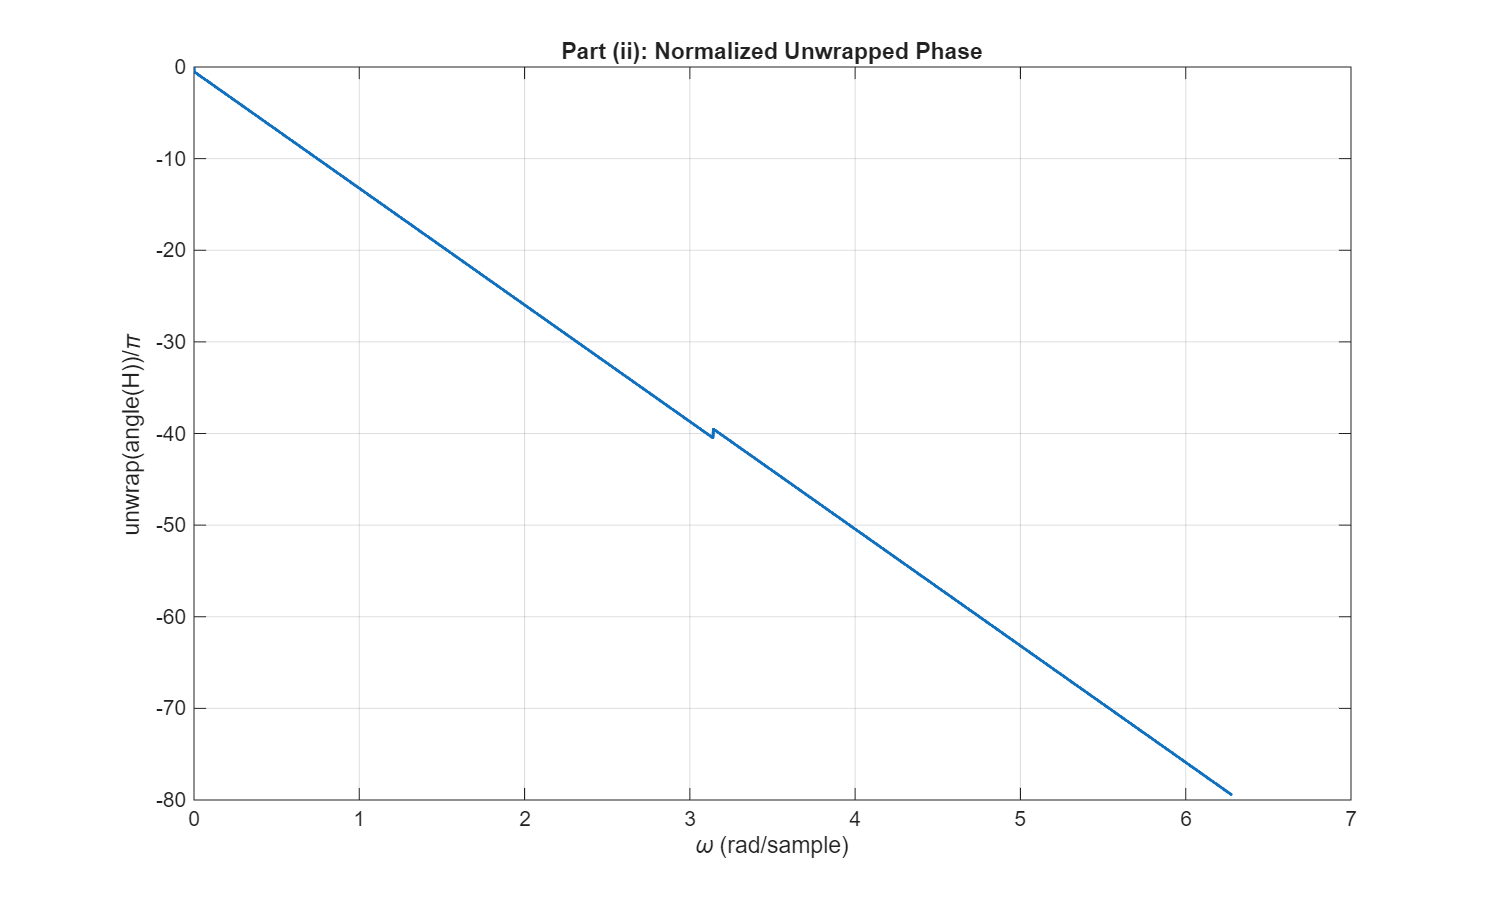
\includegraphics[width=0.85\textwidth]{part2_phase.png}
\end{figure}

% =========================
\section*{Part (iii)}
\begin{boxstyle}
Signal band within 60 dB: $[0, 5500]$ Hz. \\
Not fully inside passband since it includes frequencies below 800 Hz.
\end{boxstyle}

\begin{figure}[H]
\centering
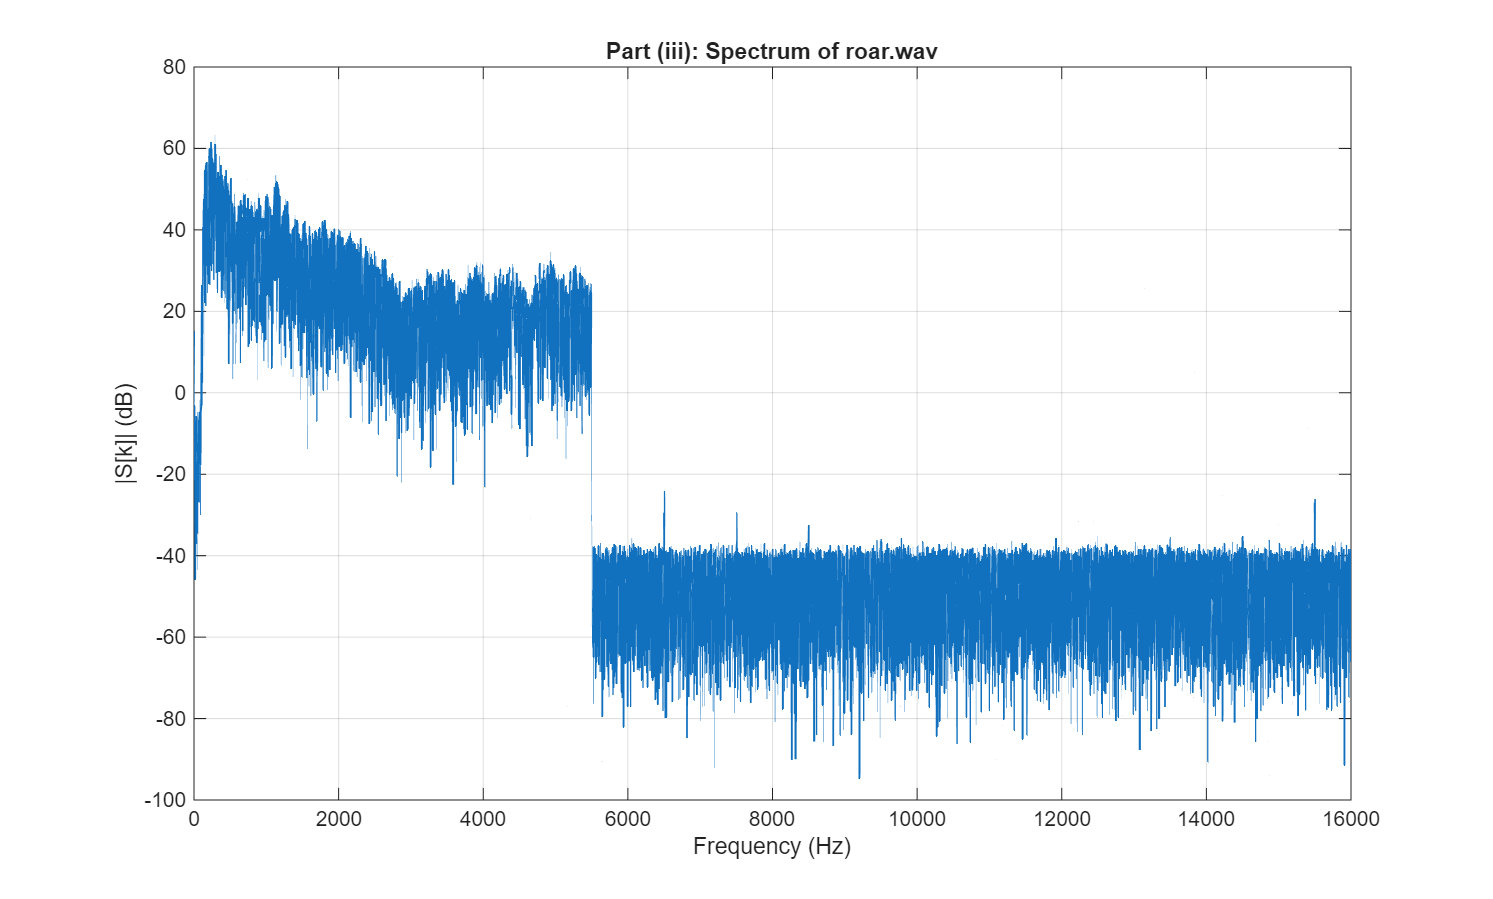
\includegraphics[width=0.85\textwidth]{part3_audio_spectrum.png}
\end{figure}

% =========================
\section*{Part (iv)}
\begin{boxstyle}
Upper sideband preserved. \\
Missing sideband energy fraction: $0.00907$.
\end{boxstyle}

\begin{figure}[H]
\centering
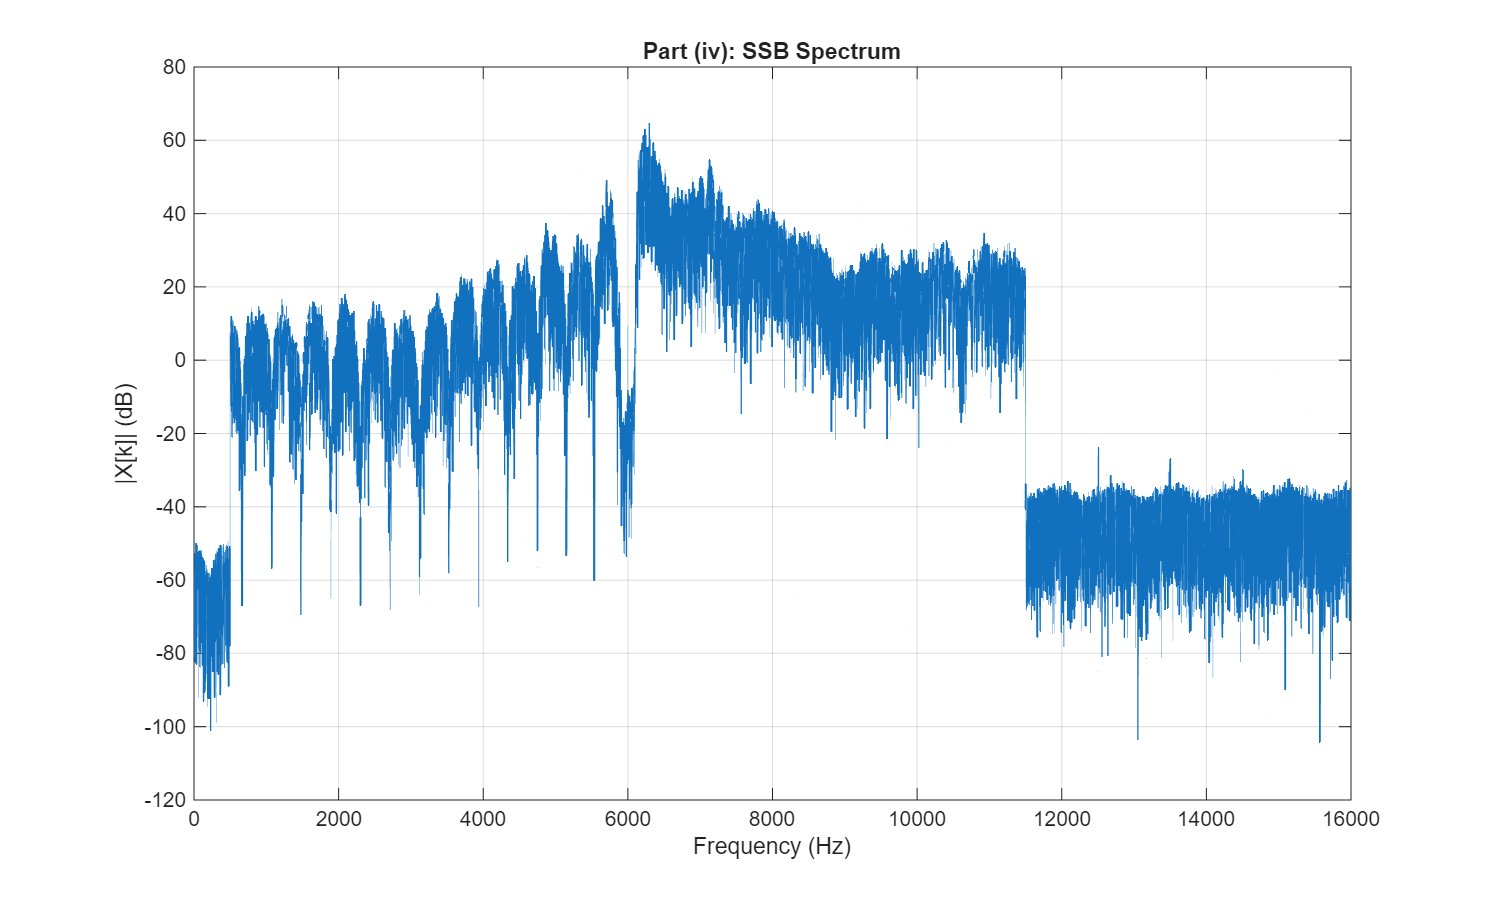
\includegraphics[width=0.85\textwidth]{part4_ssb_spectrum.png}
\end{figure}

% =========================
\section*{Part (v)}
\begin{boxstyle}
Demodulated signal differs from original. \\
Relative error: $0.50407$.
\end{boxstyle}

\begin{figure}[H]
\centering
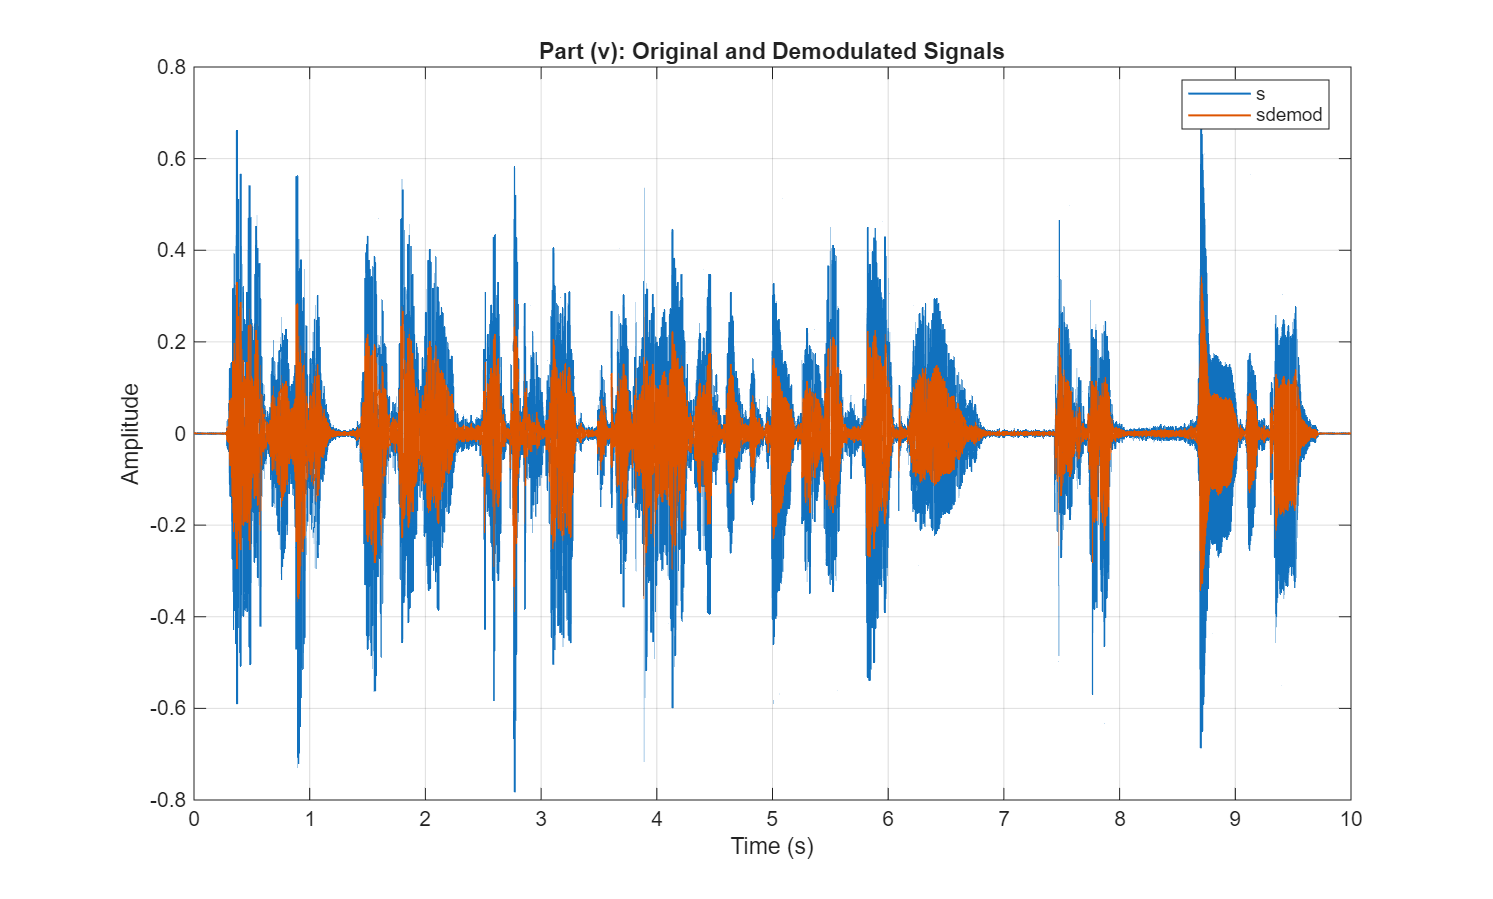
\includegraphics[width=0.85\textwidth]{part5_demod_compare.png}
\end{figure}

\end{document}
